% !TeX program = pdfLaTeX
\documentclass[12pt]{article}
\usepackage{amsmath}
\usepackage{graphicx,psfrag,epsf}
\usepackage{enumerate}
\usepackage{natbib}
\usepackage{textcomp}
\usepackage[hyphens]{url} % not crucial - just used below for the URL
\usepackage{hyperref}

%\pdfminorversion=4
% NOTE: To produce blinded version, replace "0" with "1" below.
\newcommand{\blind}{1}

% DON'T change margins - should be 1 inch all around.
\addtolength{\oddsidemargin}{-.5in}%
\addtolength{\evensidemargin}{-.5in}%
\addtolength{\textwidth}{1in}%
\addtolength{\textheight}{1.3in}%
\addtolength{\topmargin}{-.8in}%

%% load any required packages here



% tightlist command for lists without linebreak
\providecommand{\tightlist}{%
  \setlength{\itemsep}{0pt}\setlength{\parskip}{0pt}}



\usepackage{booktabs}
\usepackage{longtable}
\usepackage{array}
\usepackage{multirow}
\usepackage{wrapfig}
\usepackage{float}
\usepackage{colortbl}
\usepackage{pdflscape}
\usepackage{tabu}
\usepackage{threeparttable}
\usepackage{threeparttablex}
\usepackage[normalem]{ulem}
\usepackage{makecell}
\usepackage{xcolor}

\begin{document}


\def\spacingset#1{\renewcommand{\baselinestretch}%
{#1}\small\normalsize} \spacingset{1}


%%%%%%%%%%%%%%%%%%%%%%%%%%%%%%%%%%%%%%%%%%%%%%%%%%%%%%%%%%%%%%%%%%%%%%%%%%%%%%

\if0\blind
{
  \title{\bf Does Not Playing Hockey Make You Worse At Hockey?
Investigating the Impact of the COVID-19 Pandemic on Hockey Player
Development}

  \author{
        Michele Sezgin \thanks{The authors gratefully acknowledge Sam
Ventura, Ron Yurko, Ben Baumer, and Ryne Vankrevelen} \\
    Department of Statistical and Data Sciences, Smith College\\
     and \\     Jackie Jovanovic \\
    Department of Statistics, Elon University\\
      }
  \maketitle
} \fi

\if1\blind
{
  \bigskip
  \bigskip
  \bigskip
  \begin{center}
    {\LARGE\bf Does Not Playing Hockey Make You Worse At Hockey?
Investigating the Impact of the COVID-19 Pandemic on Hockey Player
Development}
  \end{center}
  \medskip
} \fi

\bigskip
\begin{abstract}
During 2020-2021, many hockey leagues had shortened seasons or no
seasons due to the restrictions on play caused by the COVID-19 pandemic.
The Ontario Hockey League did not play any games during this ``COVID''
season, which raises the question of whether not playing games during
the 2020-2021 COVID season negatively impacted player development (or
even caused players to get worse). Statistical and causal inference
methods were employed to assess the impact of not playing during the
COVID season, including Ordinary Least Squares, Gamma, Mixed Effects,
and matched regression models, as well as a Bayesian Additive Regression
sum of Trees model. All models pointed to no significant difference in
post-COVID performance for treated (played during COVID season) vs
control (did not play during COVID season) groups. Future research
should focus on studying other populations, experimenting with
alternative variable definitions, and studying player development curves
to more thoroughly assess treatment impact.
\end{abstract}

\noindent%
{\it Keywords:} sports analytics, causal inference, Coronavirus pandemic
\vfill

\newpage
\spacingset{1.45} % DON'T change the spacing!

\hypertarget{introduction}{%
\section{Introduction}\label{introduction}}

During 2020-2021, many hockey leagues had shortened seasons or no
seasons due to the restrictions on play caused by the COVID-19 pandemic.
Among these leagues were National Hockey League (NHL) feeder leagues,
such as the Ontario Hockey League (OHL), the Western Hockey League, and
the Quebec Major Junior Hockey League. Some players experiencing
restrictions on play participated in other leagues or tournaments during
the 2020-21 season, while others did not. This raises the question of
whether not playing games during the 2020-2021 COVID season negatively
impacted player development (or even caused players to get worse).

To answer this question, we examined data from the OHL, which did not
play any games during the 2020-21 season due to the state of the
COVID-19 pandemic (1). Some players from this league found leagues
abroad (U.S. or Europe) to play in, while others recorded no games
during 2020-2021, which we will call the COVID season. While some
leagues may have played a partial season, OHL players either played in
another league, or they did not play at all. This provided a natural
experiment, allowing us to not only use traditional statistical
inference but also causal inference methods.

There has been much speculation from coaches, scouts, sports
commentators, and fans about the effects of the COVID season on player
development \cite{sportsnet, traikos}. The question many asked prior to
the COVID season remains (at least quantitatively) unanswered: ``what
will be the impact on athletes unable to compete for well over a year
during a key stretch of their development?'' \citet{sportsnet}. Some
coaches theorized that players would become better and stronger having
had time off to reevaluate their individual performance and work on more
skill, speed, and strength training \citet{sportsnet}, while others
feared the lack of game play may have dulled the sharpening hockey
skills and IQ of developing players \citet{traikos}. There have been
plenty of skaters who had to take time off from their hockey career due
to injury and came back better and stronger than before
\cite{dixon, kreiser}. However, these are typically NHL players with
access to extensive training and rehabilitation resources, something
that not all OHL players may have had. Additionally, these players are
typically not taking time off during pivotal developmental years; they
are already well-established professional players.

\hypertarget{previous-work}{%
\section{Previous Work}\label{previous-work}}

Previous work in this area has investigated the impact of injury on
player development and important psychological aspects of player
development. Much work has focused on psychological aspects in player
development, such as mutual trust and respect between athletes and their
coaches, or frameworks through which players develop
\cite{lefebvre, soberlak}. But little research was found on pivotal
developmental years or typical development curves for ice hockey
players, though some work has been done to investigate development
progression in swimming \citet{born}. This research pointed to
significant development from ages 10 to roughly 17 depending on the
group analyzed, which could potentially translate to hockey development
and OHL players. The prior research most similar to our research
investigated the performance impacts of concussions in the NHL
\cite{buckley, neustadtl}. Neustadtl et al.~found no significant
differences in pre- and post-concussion performance for the 269 NHL
players studied. Buckley at al.~again found no significant difference in
pre and post- performance for players who missed playing time due to
injury and those who missed playing time due to non-injury reasons.
However, no research was found investigating the impact of reduced
playing time in developing (major junior) hockey players.

\hypertarget{data}{%
\section{Data}\label{data}}

Our dataset includes skaters (excludes goalies) who played in the
Ontario Hockey League (OHL) during both the pre-COVID (2019-2020) and
post-COVID (2021-2022) seasons. The dataset also contains information
regarding other leagues they have participated in during their career.
There is data about season, team, league, points, games played,
position, and drafted status. Each row is a player on a certain team in
a specific season. There are 219 observations in the dataset. The data
was sourced from Elite Prospects and was supplied by our external
advisor, Dr.~Sam Ventura.

\begin{table}

\caption{\label{tab:sample-rows}Sample data rows and variables}
\centering
\resizebox{\linewidth}{!}{
\begin{tabular}[t]{l|l|l|r|r|r|l|r}
\hline
first\_name & last\_name & position & ppg\_19 & gp\_21 & age\_continuous & treatment & ppg\_21\\
\hline
Shane & Wright & F & 1.1379310 & 63 & 15.98904 & Played & 1.492063\\
\hline
Logan & Mailloux & D & 0.0000000 & 12 & 16.71311 & Played & 0.750000\\
\hline
Wyatt & Johnston & F & 0.5660377 & 68 & 16.63388 & Played & 1.823529\\
\hline
Brandt & Clarke & D & 0.6666667 & 55 & 16.89315 & Played & 1.072727\\
\hline
\end{tabular}}
\end{table}

\hypertarget{added-variables}{%
\subsection{Added Variables}\label{added-variables}}

If a skater played for several teams during one season, including the
COVID season, the team for which they played the most games was
selected. Statistics for all other teams were dropped. This was done to
control for team effect on performance.

\(\hspace{-0.25in}\)\textbf{Player performance}: To approximate player
performance in the post-COVID season, we calculated each player's points
per game (PPG) as PPG = (goals + assists)/games played in the post-COVID
season.

\(\hspace{-0.25in}\)\textbf{Previous player performance}: To approximate
player performance in the pre-COVID season, we computed each player's
PPG in the pre-COVID season.

\(\hspace{-0.25in}\)\textbf{Treatment}: We defined a player as treated
if they participated in at least one game during the post-COVID season.
This allowed us to retain players who recorded relatively few games in
elite competitions like the International Ice Hockey Federation World
Junior Championship as treated. Thus ensuring we were not obscuring the
effects of these competitions on development. There are 67 treated
players and 152 control players.

\(\hspace{-0.25in}\)\textbf{Age}: We defined age as the continuous age
of the player as of January 1st, 2020. Previous Player Performance : To
control for player performance in the pre-COVID season, we approximated
player performance using player PPG in the pre-COVID season.

\(\hspace{-0.25in}\)\textbf{Drafted}: Whether a player was drafted in
2020 or earlier Relative PM : Relative plus-minus (PM) is defined as a
player's PM relative to the average PM of their team.

\(\hspace{-0.25in}\)\textbf{Ranked PM}: Ranked plus-minus defines how a
player's PM ranks among those of their teammates. If there are n players
on a team, each player will receive a PM ranking 1-n.

\hypertarget{data-integrity}{%
\subsection{Data Integrity}\label{data-integrity}}

Through analysis and comparison with OHL records, we estimate that we
have 99\% of the data from the 2019-2020 and 2021-2022 regular seasons
(Table 3).

\begin{table}

\caption{\label{tab:data-integrity}Missing goals for each OHL team in the 2019-2020 and 2021-2022 regular seasons}
\centering
\resizebox{\linewidth}{!}{
\begin{tabular}[t]{l|r|r|r|r|r|r}
\hline
team\_name & goals\_19 & true\_goals\_19 & difference\_19 & goals\_21 & true\_goals\_21 & difference\_21\\
\hline
Ottawa 67's & 293 & 296 & 3 & 194 & 199 & 5\\
\hline
Saginaw Spirit & 289 & 289 & 0 & 231 & 234 & 3\\
\hline
Flint Firebirds & 272 & 274 & 2 & 285 & 286 & 1\\
\hline
London Knights & 265 & 265 & 0 & 260 & 264 & 4\\
\hline
Kitchener Rangers & 260 & 264 & 4 & 235 & 236 & 1\\
\hline
Sudbury Wolves & 258 & 259 & 1 & 221 & 223 & 2\\
\hline
Soo Greyhounds & 252 & 253 & 1 & 293 & 295 & 2\\
\hline
Windsor Spitfires & 252 & 256 & 4 & 302 & 305 & 3\\
\hline
Peterborough Petes & 250 & 250 & 0 & 239 & 240 & 1\\
\hline
Sarnia Sting & 243 & 244 & 1 & 233 & 234 & 1\\
\hline
Owen Sound Attack & 233 & 235 & 2 & 233 & 235 & 2\\
\hline
Hamilton Bulldogs & 232 & 235 & 3 & 296 & 300 & 4\\
\hline
Oshawa Generals & 228 & 229 & 1 & 209 & 215 & 6\\
\hline
Erie Otters & 227 & 229 & 2 & 222 & 223 & 1\\
\hline
Mississauga Steelheads & 220 & 223 & 3 & 228 & 229 & 1\\
\hline
Barrie Colts & 217 & 220 & 3 & 243 & 245 & 2\\
\hline
Guelph Storm & 214 & 218 & 4 & 249 & 251 & 2\\
\hline
Kingston Frontenacs & 195 & 198 & 3 & 281 & 285 & 4\\
\hline
Niagara IceDogs & 191 & 194 & 3 & 212 & 218 & 6\\
\hline
North Bay Battalion & 189 & 189 & 0 & 264 & 267 & 3\\
\hline
\end{tabular}}
\end{table}

\hypertarget{eda}{%
\subsection{EDA}\label{eda}}

\hypertarget{preliminary-visualizations}{%
\subsubsection{Preliminary
Visualizations}\label{preliminary-visualizations}}

The distribution of player performance is right-skewed, showing that
most players do not generate many points per game. The preliminary
hypothesis that not playing during the COVID season negatively impacted
player performance is motivated by the plot of player performance
distributions conditioned on treatment. It appears that players who
played during the COVID season performed better in the post-COVID
season, which motivated our analysis. Our models attempt to tease out if
this difference is ``real''. \(\\\)

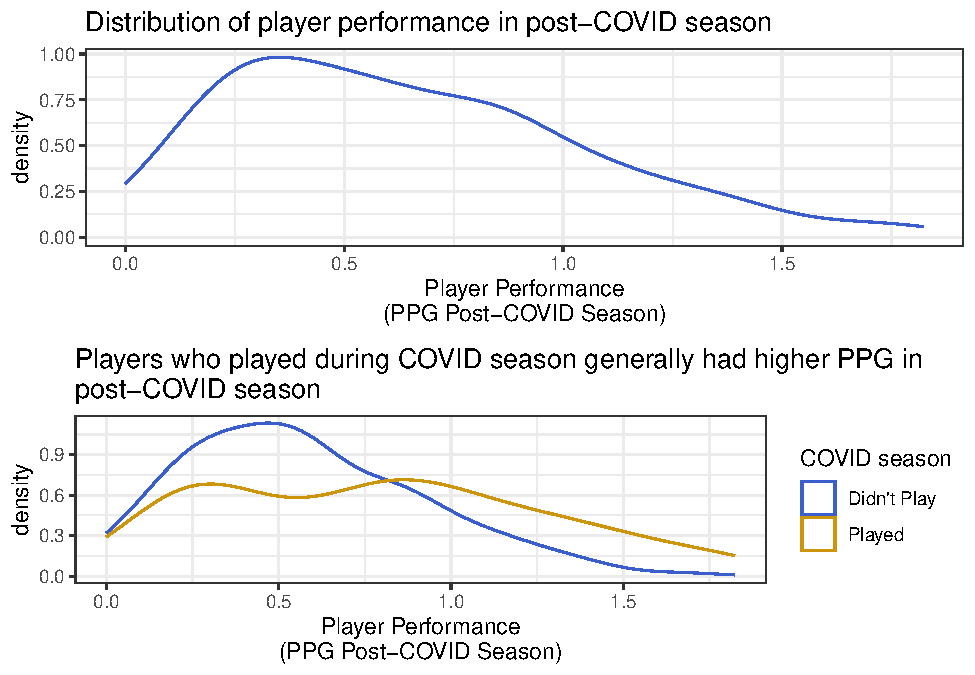
\includegraphics{journal-article_files/figure-latex/prelim-plots-1.pdf}
\(\hspace*{\fill} \footnotesize \text{Figure 1. preliminary visualizations}\)

We investigated relationships between potential confounders and our
treatment and response to aid in variable selection. The variables we
hypothesized as potential confounders are age, games played, drafted
status, previous player performance, and position.

\hypertarget{age}{%
\subsubsection{Age}\label{age}}

We hypothesized that older players would be more likely to have better
player performance, because they are further along in their development.
Interestingly, the below plots do not support a strong relationship
between age and player performance. We additionally hypothesized that
older players would be more likely to be treated using the same logic as
before. Better players are more likely to be selected to play in
leagues, and older players tend to be better. However, the distributions
do not differ significantly when conditioning on treatment. \(\\\)

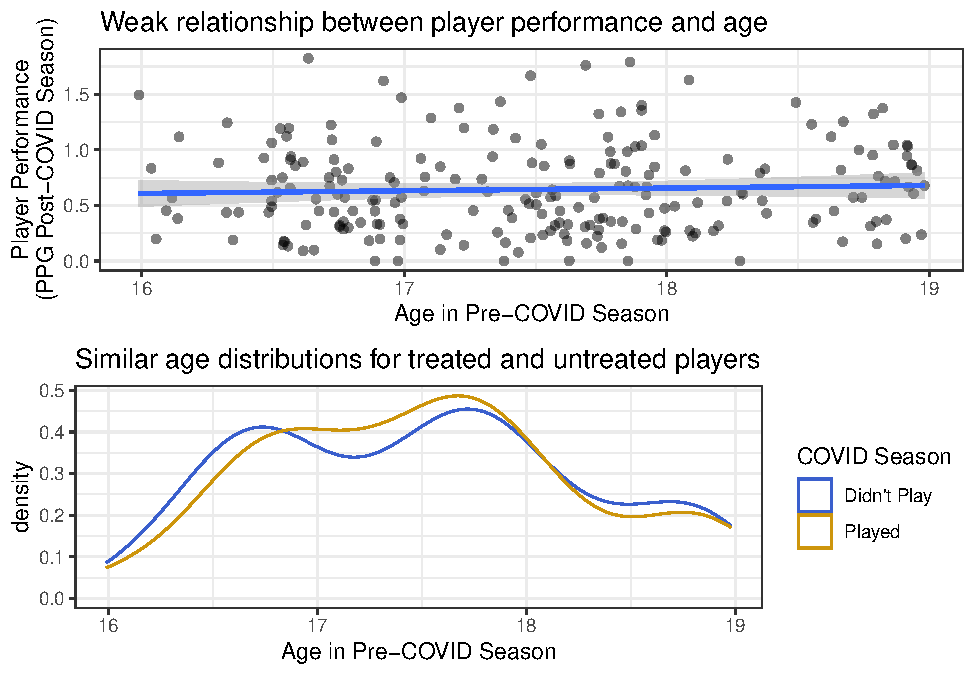
\includegraphics{journal-article_files/figure-latex/age-plots-1.pdf}
\(\hspace*{\fill} \footnotesize \text{Figure 2. age vs. treatment and response}\)

\hypertarget{games-played}{%
\subsubsection{Games Played}\label{games-played}}

The data supports that players who play more games are likely to be
higher performing players. I.e. ``good players don't get benched'', as
expected. However, there are no overwhelming differences in the
distributions of player performance when conditioning on treatment, and
the instability in the distribution of player performance for players
who played during the COVID season is likely due to the smaller sample
size.

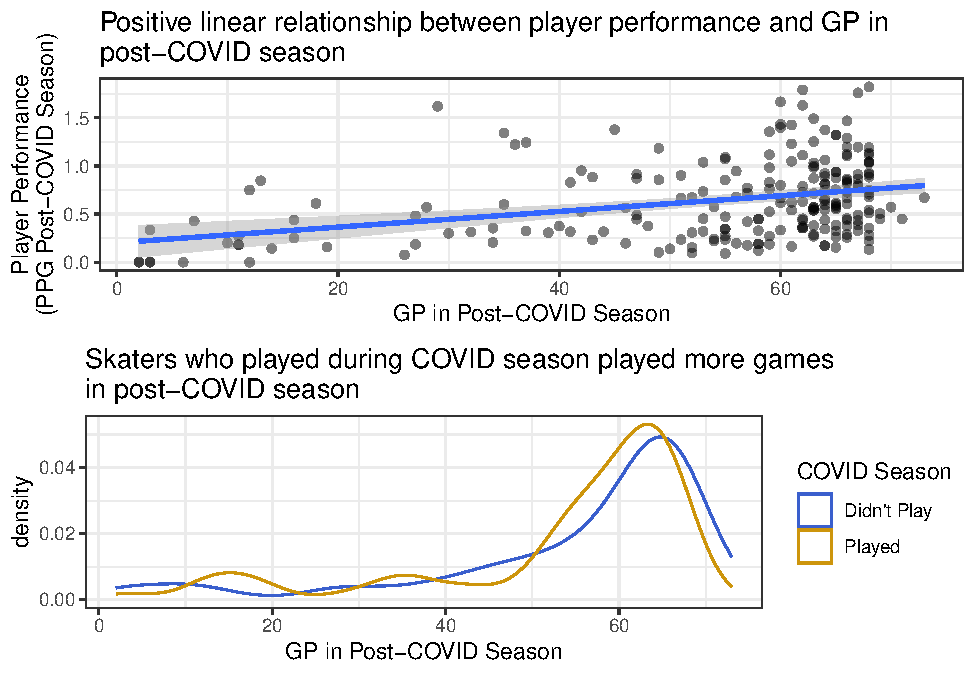
\includegraphics{journal-article_files/figure-latex/gp-plots-1.pdf}
\(\hspace*{\fill} \footnotesize \text{Figure 3. games played vs. treatment and response}\)

\hypertarget{previous-player-performance}{%
\subsubsection{Previous Player
Performance}\label{previous-player-performance}}

We hypothesized that higher performing players pre-COVID would likely be
higher performing players post-COVID, because good players tend to keep
being good. The data supports that there is a positive, moderate linear
relationship between previous player performance and post-COVID player
performance. We additionally thought that higher performing players
pre-COVID would be more likely to be treated, because it would be easier
to convince overseas leagues to take on better players, a notion that
appears to be supported by the data.

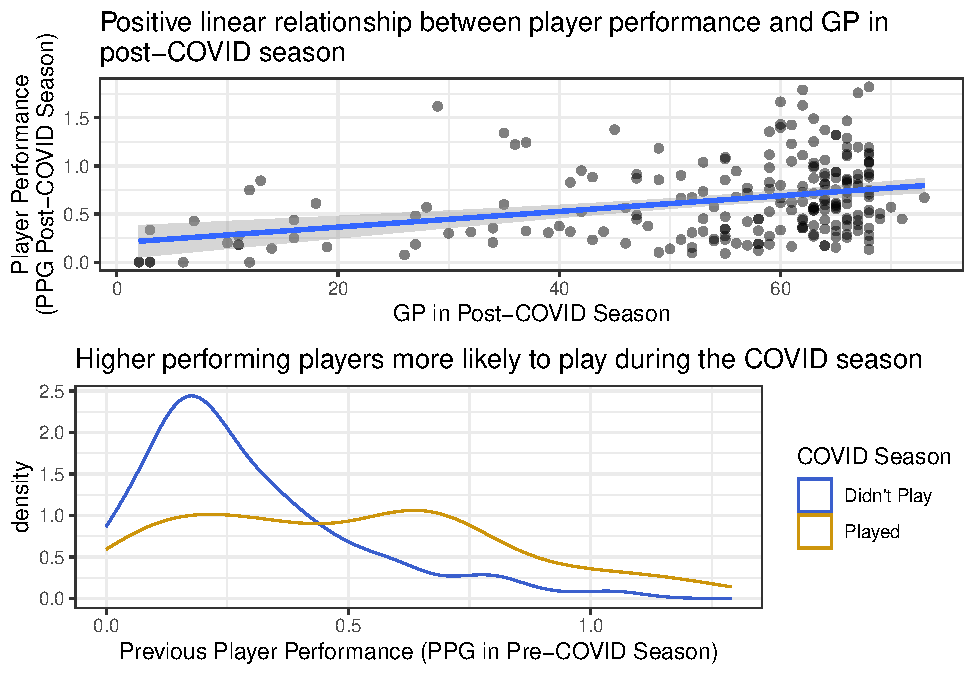
\includegraphics{journal-article_files/figure-latex/ppp-plots-1.pdf}
\(\hspace*{\fill} \footnotesize \text{Figure 4. previous player performance vs. treatment and response}\)

\hypertarget{position}{%
\subsubsection{Position}\label{position}}

Lastly, we know that defensemen will be lower performing players because
of the way we have defined player performance and because of the nature
of the position, a notion that is supported by the data. However, there
is no reason to believe that position would influence probability of
treatment, which is again supported by the data.

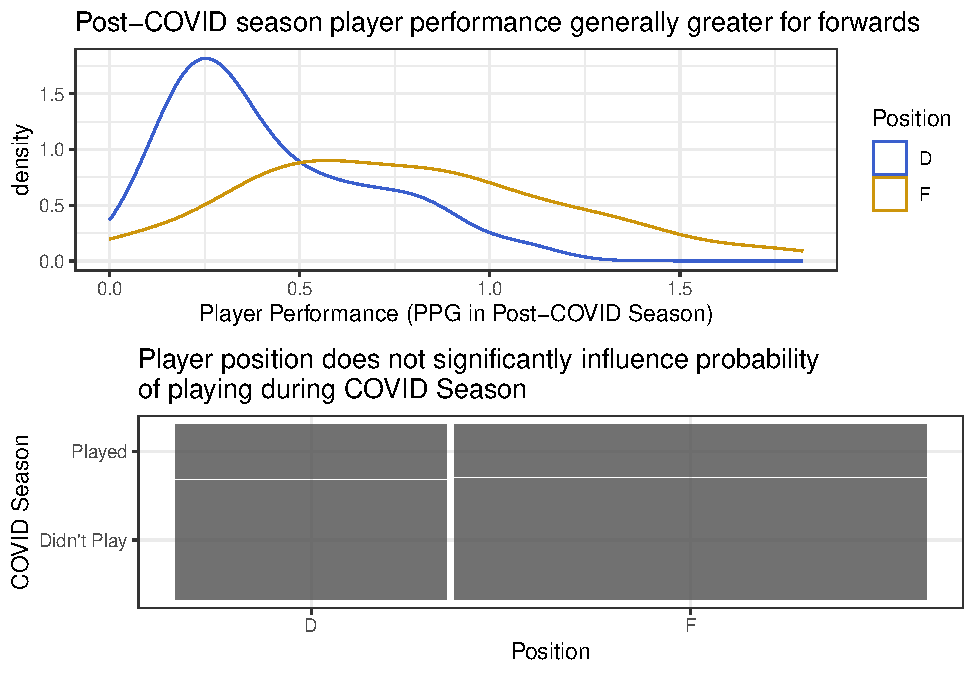
\includegraphics{journal-article_files/figure-latex/pos-plots-1.pdf}
\(\hspace*{\fill} \footnotesize \text{Figure 5. position vs. treatment and response}\)

\hypertarget{methods}{%
\section{Methods}\label{methods}}

Before performing causal analysis, we used traditional statistical
inference methods to determine whether playing during the COVID season
had a significant effect on post-COVID player performance while
controlling for variables (and interactions between variables) suspected
to be associated with the response through exploratory data analysis
(EDA). When possible, we attempted a few different measures of player
performance, including PPG z-scores (to control for differences in
overall scoring across seasons) and relative plus-minus scores. All code
is available in the supplementary code document of the supplementary
materials folder \citet{sezgin}.

For all methods \(\epsilon \sim N(0, \sigma^2)\)

\hypertarget{regression}{%
\subsection{Regression}\label{regression}}

\hypertarget{ols}{%
\subsubsection{OLS}\label{ols}}

We fit an Ordinary Least Squares (OLS) regression model without
interaction, because it is the simplest and most interpretable model to
assess the significance of playing during COVID, while still controlling
for variables that could be confounding our analysis.

\vspace{-.5cm}

\[\text{Player Performance} = \beta_0 + \beta_1\text{Treatment} + \beta_2\text{Forward} +  \beta_3\text{Previous Performance} \hspace{.1cm} + \]
\[\beta_4\text{Games Played Post-COVID} + \beta_5\text{Age} + \epsilon\]

\hypertarget{interaction-ols}{%
\subsubsection{Interaction OLS}\label{interaction-ols}}

We fit an OLS model with interaction to account for relationships
observed between explanatory variables during the EDA process. We also
tested whether the additional complexity of this full model
significantly increased predictive power over the nested model.

\vspace{-.5cm}

\[\text{Player Performance} = \beta_{0} + \beta_{1}\text{Treatment} + \beta_{2}\text{Forward} +  \beta_{3}\text{Previous Performance} \hspace{.1cm} +\]
\[\beta_{4}\text{Games Played Post-COVID} + \beta_{5}\text{Age} + \beta_{6}\text{Position*Previous Performance} \hspace{.1cm} + \]
\[\beta_{7}\text{Age*Previous Performance} + \beta_{8}\text{Previous Performance*Treatment} + \beta_{9}\text{Games Played} + \epsilon\]

\hypertarget{gamma}{%
\subsubsection{Gamma}\label{gamma}}

PPG is right skewed and bounded between 0 and some positive number, so
we believed PPG may be Gamma-distributed. We performed simple and
interaction Gamma regression with the log link function in an attempt to
more accurately model the relationship between our response and
explanatory variables.

\vspace{-.5cm}

\begin{itemize}
\tightlist
\item
  \(\text{Player Performance} \sim \text{Gamma}(\alpha, \lambda)\)
\item
  \(\text{for the }i^{th} \text{player, } i= 1,..., 219,\)
  \[E[\text{Player Performance}_{i}] =  e^{\beta_0} \text{Treatment}^{\beta_1}  \text{Forward}^{\beta_2} \text{Previous Performance}^{\beta_3}\]
  \[\text{Games Played Post-COVID}^{\beta_3} \text{Age}^{\beta_5}\]
\end{itemize}

\hypertarget{mixed-effects-model}{%
\subsubsection{Mixed-effects Model}\label{mixed-effects-model}}

Lastly, we fit a mixed-effects model to determine if the effect of
playing during the COVID season was significantly different across
leagues. The slope and intercept of the regression line varied according
to the league. Players who did not participate during the COVID season
were grouped into a ``league'' called ``NONE''.

\textbf{Level One}:

\begin{itemize}
\tightlist
\item
  \(\text{for the }i^{th} \text{player, } i= 1,..., 219,\)
\end{itemize}

\[Y_i = a_i + b_i\text{Treatment} + \epsilon_i\]

\begin{itemize}
\tightlist
\item
  \(\epsilon_i \sim N(0, \sigma^2)\)
\end{itemize}

\textbf{Level Two}:

\begin{itemize}
\item
  \(a_i = \alpha_0 + \alpha_1\text{Forward} + \alpha_2\text{Previous Performance} + \alpha_3\text{Games Played Post-COVID} + \alpha_4\text{Age} + u_i\)
\item
  \(b_i = \beta_0 + \beta_1\text{Forward} + \beta_1\text{Previous Performance} + \beta_3\text{Games Played Post-COVID} + \beta_4\text{Age} + v_i\)
\end{itemize}

\begin{align*}
\begin{bmatrix}u_{i}\\
v_{i}
\end{bmatrix} &\sim  N
\begin{pmatrix}
\begin{bmatrix}
0\\
0
\end{bmatrix}\!\!,&
\begin{bmatrix}
\sigma_{u}^2 & \\
\rho\sigma_{u}\sigma_{v} & \sigma_{v}^2
\end{bmatrix}
\end{pmatrix}
\end{align*}

\hypertarget{causal-methods}{%
\subsection{Causal Methods}\label{causal-methods}}

\hypertarget{matching}{%
\subsubsection{Matching}\label{matching}}

Matching on covariates allowed us to better control for confounding
variables and more accurately estimate the true impact of the treatment.
The results fit on matched data were compared to the results of the
model fit on unmatched data. Control and treatment observations were
matched on games played post-COVID, position, points pre-COVID, previous
player performance, age, and ranked PM pre-COVID. ``Optimal'' matching
method and GAM measure of distance were used, and a 1-to-1 matching
ratio was used due to the small sample size. The model is the same as
the OLS model, but fit with matched data.

\hypertarget{bart}{%
\subsubsection{BART}\label{bart}}

An appeal of the Bayesian Additive Regression Trees (BART) model is that
it controls overfitting, which is one issue with normal additive
regression trees. Each tree tries to account for something new in the
model. Once all added, accurate estimates are produced. This allows for
causal inferences to be drawn. The workflow used is taken from Joshua
Bon's vignette on using the tidytreatment package with BART.

A variable selection model was used to find important variables for
obtaining propensity scores. The variable selection model was a
continuous BART model regressing all covariates except for the treatment
against post-COVID player performance. The burn-in period was set to
2000 iterations, with posterior draws set to 5000. Variables were deemed
important if their average inclusion in the model was equal to or
greater than 50\%. The most important variables were used to produce
propensity scores using a probit BART model, with a burn-in of 2000
draws and 5000 posterior draws. Finally, all covariates, including
treatment, and propensity scores were used in the final BART model to
predict post-COVID player performance. The final model produced a
posterior distribution of estimated post-COVID player performance for
each player, with a burn-in of 10,000 draws and 200 posterior draws per
player. The method of obtaining the posterior is outlined by
\citet{chipman}.

For all models ``let \(T\) denote a binary tree consisting of a set of
interior node decision rules and a set of terminal nodes, and let
\(M = \{\mu_1, \mu_2, . . . ,\mu_b\}\) denote a set of parameter values
associated with each of the \(b\) terminal nodes of \(T\)''
\citet{chipman}.

\textbf{Variable selection model}:

\[\text{Player Performance} = \sum_{j=1}^{25} g(x;T_{j}, M_{j}) + \epsilon\]

\begin{itemize}
\item
  \(x = \{ \text{Games Played Pre-COVID}, \text{Games Played Post-COVID}, \text{Points Pre-COVID}, \text{Age}, \\ \text{Ranked PM Pre-COVID}, \text{Relative PM Pre-COVID}, \text{PM Pre-COVID}, \text{Position}, \\ \text{Previous Player Performance} \}\)
\item
  \(x_{important}\) are the most variables in this model, deemed
  important if average inclusion was greater than or equal to 50\%.
\end{itemize}

\textbf{Propensity score model}:

\vspace{-.5cm}

\[\text{Propensity Score} = P(\text{Treatment} = \text{played } | \hspace{.1cm} x_{important}) = \Phi(\sum_{j=1}^{200} g(x_{important};T_{j}, M_{j}) + \epsilon)\]

\begin{itemize}
\tightlist
\item
  \(\Phi\) is the cumulative distribution function of the standard
  normal distribution.
\end{itemize}

\textbf{Final Predictive Model}:

\[ \text{Player Performance} = \sum_{j=1}^{200} g(x, \text{Treatment}, \text{Propensity Score};T_{j}, M_{j}) + \epsilon\]

\hypertarget{results}{%
\section{Results}\label{results}}

Across all models there was no evidence of a treatment effect given the
observed data, regardless of the measure of player performance chosen
(PPG, PPG z-scores, ranked PM, relative PM). PPG was ultimately chosen
as the response measure because of its interpretability. The root mean
squared error (RMSE) values for each of the models according to
ascending error is summarized in Table 3.

\begin{table}

\caption{\label{Table 3.}RMSE values for all models}
\centering
\begin{tabular}[t]{l|r}
\hline
model & RMSE\\
\hline
BART & 0.2254971\\
\hline
mixed effects & 0.2386779\\
\hline
OLS interaction & 0.2548995\\
\hline
OLS & 0.2553530\\
\hline
intercept-only & 0.2662603\\
\hline
matched & 0.4018033\\
\hline
gamma simple & 1.1395561\\
\hline
gamma interaction & 1.2248592\\
\hline
\end{tabular}
\end{table}

\hypertarget{regression-1}{%
\subsection{Regression}\label{regression-1}}

The regression model that best balances accuracy and parsimony is the
OLS model.

\(\widehat{\text{Player Performance}} = 1.14 + 0.05*\text{Treatment} + 0.18*\text{Forward} + 0.89*\text{Previous Performance} \hspace{.1cm} + .006*\text{Games Played Post-COVID} - .07*\text{Age}\)
\(\vspace{.25cm}\)

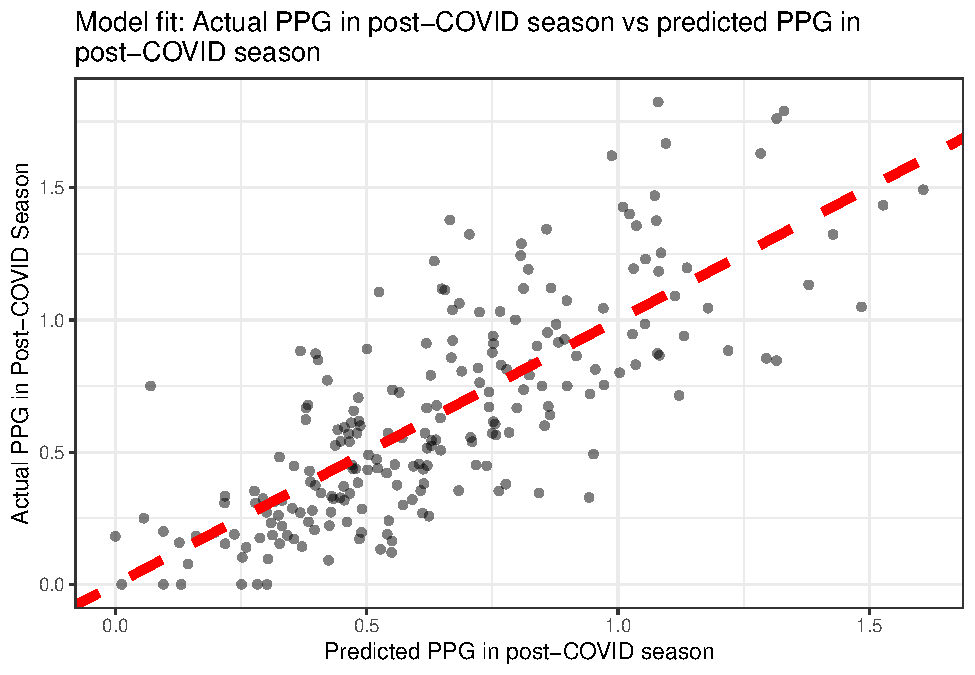
\includegraphics{journal-article_files/figure-latex/ols-plot-1.pdf}

\begin{itemize}
\item
  Coefficients for position, games played in post-COVID season, age, and
  previous player performance were all found to be statistically
  significant from 0 at the \(\alpha = 0.01\) level.
\item
  The model explains approximately 59\% of the variation in player
  performance in the post-COVID season, which is a statistically
  significant amount at the \(\alpha = .001\) level
  \(F(5, 213) = 62.88, p<.001\).
\end{itemize}

\hypertarget{bart-1}{%
\subsection{BART}\label{bart-1}}

The variables deemed important in the variable selection model were
games played post-COVID, points pre-COVID, relative PM pre-COVID,
position, and previous player performance.

\(x_{important} = \{ \text{Games Played Post-COVID}, \text{Points Pre-COVID}, \text{Age}, \\ \text{Relative PM Pre-COVID}, \text{Position}, \text{Previous Player Performance}\}\)
\(\vspace{.25cm}\)

The estimated effects do not differ significantly from the line at 0,
which indicates that there is not sufficient evidence of a treatment
effect. The histogram of treatment effects is bell-shaped and fairly
symmetric. The mean treatment effects show that there could be a
slightly positive, though extremely small treatment effect for all
subjects, but this is shown to be not significant in Figure 7.

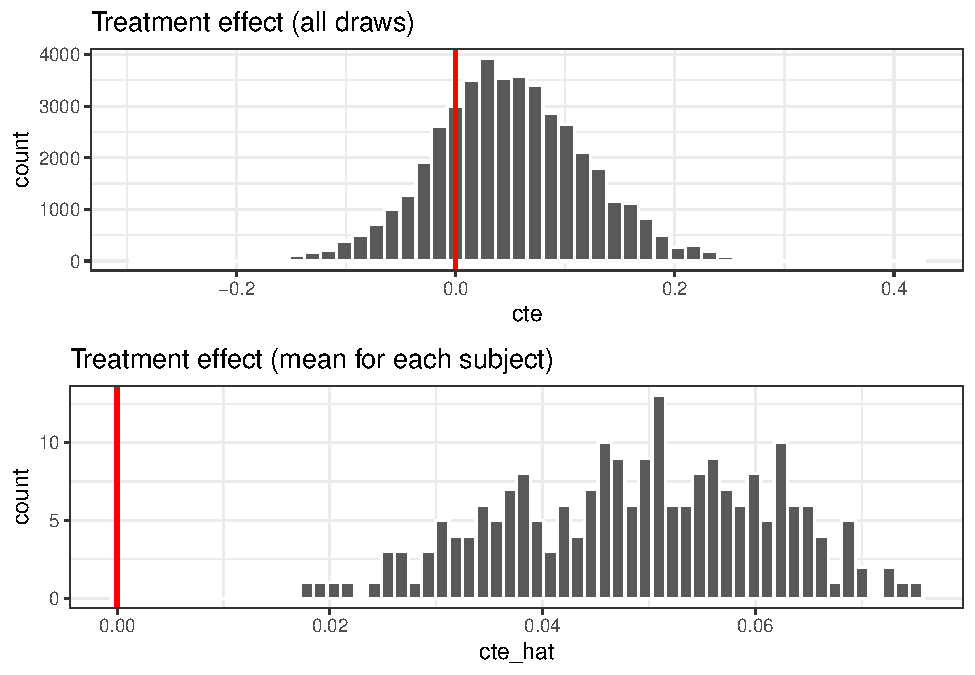
\includegraphics{journal-article_files/figure-latex/bart-plots-1.pdf}
\(\hspace*{\fill} \footnotesize \text{Figure 6. BART posterior draws and means plots}\)

The confidence intervals for Conditional Average Treatment Effect
support the same conclusions. Similar to the mean treatment effects,
most of the point estimates in Figure 7 are positive. But since all of
the confidence intervals contain 0, this visualization is compatible
with no treatment effect.

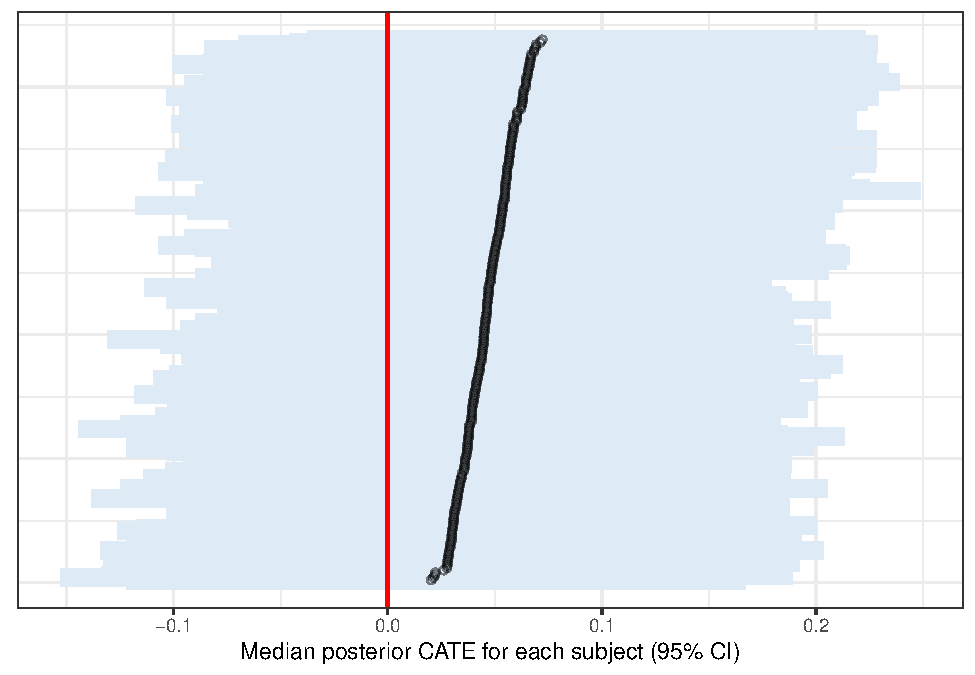
\includegraphics{journal-article_files/figure-latex/bart-cates-1.pdf}
\(\hspace*{\fill} \footnotesize \text{Figure 7. BART CATE plot}\)

\hypertarget{discussion}{%
\section{Discussion}\label{discussion}}

\hypertarget{interpretations-of-models}{%
\subsection{Interpretations of Models}\label{interpretations-of-models}}

\hypertarget{ols-regression-model}{%
\subsubsection{OLS Regression Model}\label{ols-regression-model}}

Player performance in the post-COVID season is expected to increase by
0.05 PPG on average for skaters who played during COVID, when holding
constant position, previous player performance, games played in the
post-COVID season, points scored in the pre-COVID season, and age. Over
the course of a 68 game season in the OHL, the treatment effect would
result in only approximately 3 extra points. In this model, the
coefficient for whether someone played during the COVID-season was not
statistically significantly different from zero. There is no evidence
that playing during the COVID season impacted player performance in the
post-COVID season for players who played in both the pre- and post-COVID
seasons in the OHL.

We are 95\% confident that the change in player performance in the
post-COVID for players who played during the COVID season is between
-0.0185 and 0.149 PPG, holding constant position, previous player
performance, games played in the post-COVID season, points scored in the
pre-COVID season, and continuous age. This model can be used to predict
player performance in the post-COVID season based on a variety of
factors in the pre-, COVID, and post-COVID seasons among skaters who
played in the OHL in both the pre- and post-COVID seasons. For example,
using Shane Wright as our observation (Table 4), the model predicts his
post-COVID player performance to be 1.61 points per game, while his
actual points per game was slightly lower at 1.49.

\begin{table}
\caption{\label{Table 4.}Shane Wright stats}
\centering
\begin{tabular}{l|l|r|r|r|r|r}
\hline
treatment & position & ppg\_19 & gp\_21 & age\_continuous & ppg\_21 & ols\_pred\\
\hline
Played & F & 1.137931 & 63 & 15.98904 & 1.492063 & 1.606924\\
\hline
\end{tabular}
\end{table}

\hypertarget{limitations}{%
\subsection{Limitations}\label{limitations}}

\hypertarget{model-limitations}{%
\subsubsection{Model Limitations}\label{model-limitations}}

\hypertarget{ols-1}{%
\paragraph{OLS:}\label{ols-1}}

The model conditions for inference were not all met. The relationship
between our explanatory variables and post-COVID season PPG looks
roughly linear, so the linearity condition of OLS is met. However, the
skaters in the dataset are playing together on the same teams in the
same league and influencing each other's player performance. Because we
were using player level data, and not play level data, we could not
attempt to account for this non-independence. Therefore, this condition
is not met. The residuals seem roughly normally distributed, as shown in
the normal QQ plot, so this condition is met. There seems to be roughly
constant variance in residuals across all levels of our explanatory
variables, so the error homogeneity condition is met.

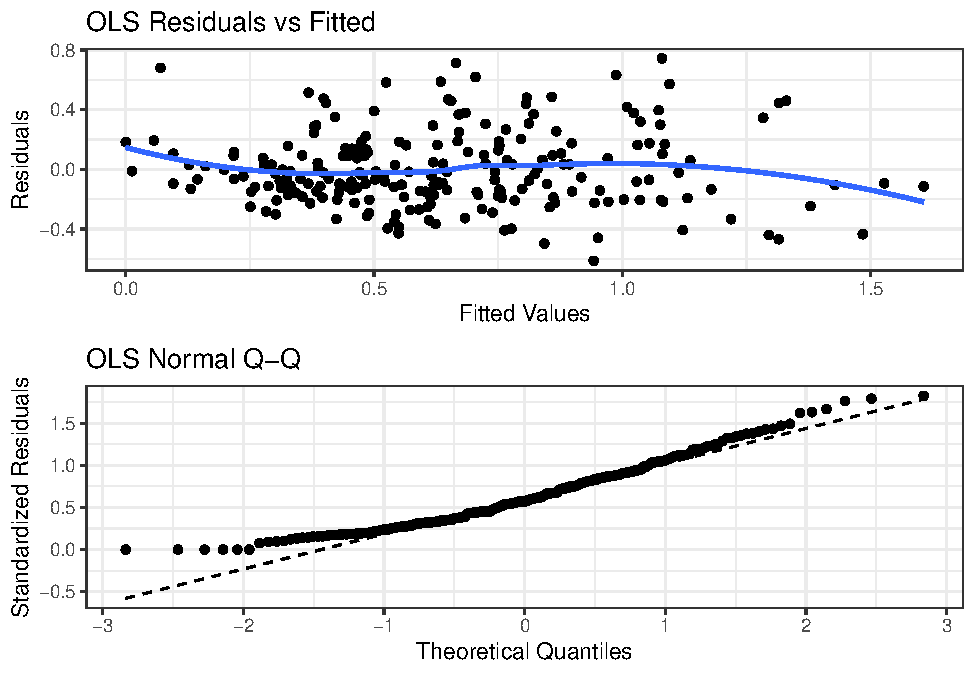
\includegraphics{journal-article_files/figure-latex/ols-limitation-plots-1.pdf}

\hypertarget{mixed-effects}{%
\paragraph{Mixed Effects}\label{mixed-effects}}

Though the mixed effects model shows a significant positive effect for
some teams, the confidence intervals were generated using as few as one
observation in many cases. Teams where a significant positive effect is
shown had at most eight observations. Because of these small sample
sizes, we did not believe that our confidence intervals nor our league
effect size estimates were credible. Additionally, the model did not
converge.

\hypertarget{matched-regression}{%
\paragraph{Matched regression}\label{matched-regression}}

Though the the regression model fit on matched data did not support a
significant treatment effect, the matching was not ideal. There were not
enough observations in the dataset to support extremely precise matching
between treatment and control units.

\hypertarget{variable-and-data-limitations}{%
\subsubsection{Variable and Data
Limitations}\label{variable-and-data-limitations}}

Though we hypothesized that drafted status would have a significant
effect on treatment status, unfortunately not enough players in our
dataset were drafted prior to the COVID season for this variable to be
meaningful (only three players were drafted pre-COVID). We hypothesized
that if a player was drafted, it is more likely that they would be able
to play during the COVID season, because their NHL team would have the
resources to convince a league or team to take the player on for that
year. Additionally, we do not have any record of players who left the
OHL post-COVID. It is possible that there are a significant number of
players who played during the COVID season and became too advanced to
continue playing in the OHL, resulting in them leaving to play in other
leagues. This missing data could be confounding our analysis, because if
these hypotheticals were true, then including these players would likely
result in the treatment effect being significantly positive.

Our estimates of player performance were biased towards offensive
production. Variables such as time on ice, line number, shots blocked,
successful passes, and battles won, among other measures could be
combined to create a more comprehensive metric to approximate player
performance, which may show a different treatment effect. In general
there are many confounding variables that were either not present in our
dataset or cannot be easily measured. For example, possible confounders
that were not measured in our dataset are time spent practicing per week
(on ice, off ice, etc), coaching support, diet, etc.

\hypertarget{future-work}{%
\section{Future Work}\label{future-work}}

Future models could utilize weighting and account for dependence of
observations. If models were weighted so that players who played more
games contributed more to the overall outcome of the model and
significance of the treatment, this would likely result in more robust
estimates of the treatment effect. Player performance for players who
only played a small number of games may not be as accurate as player
performance for players with more games. Additionally, robust variances
could be used when performing inference for models because of the
dependence of our residuals. Play-level data could also be used to
address the dependence of residuals in the dataset.

Ideally, we would like to study the effects of the COVID-19 pandemic
restrictions and prolonged periods without play on other populations.
For example, we would like to investigate if our results generalize to
goalies, other major junior leagues, and the NHL/NHL taxi squad. There
are other scenarios where players experienced prolonged periods without
play. Players may be forced to take time off due to injury, personal
reasons, or scenarios like the NHL lockouts.

We would also like to facilitate a comparison of typical hockey player
development curves compared to COVID-impacted development curves, and
investigate the impact of our treatment on long-term development. Even
if not playing during the COVID season negatively impacted the
development of any population of players, would this impact last
forever? Or is it the case that these players would catch up to their
counterparts who played during the COVID season in the long-term? As
time passes and more data is collected post-COVID, future work could
focus on assessing the long-term impact of playing or not playing during
the COVID season or not playing during other seasons.

\hypertarget{conclusion}{%
\section{Conclusion}\label{conclusion}}

When studying the effects of the pandemic hockey restrictions on OHL
hockey player performance, no significant effect was found between those
who played during the pandemic and those who didn't. Both statistical
and causal inference methods showed no significant evidence of a
treatment effect when controlling for relevant confounding variables,
though model and data limitations may have contributed to this null
effect. Further research could investigate other populations and
variable definitions to determine if our results generalize beyond the
population studied.

\hypertarget{acknowledgments}{%
\section{Acknowledgments}\label{acknowledgments}}

Thank you to our external advisors, professors, and universities, we
could not have completed this project without them and we sincerely
appreciate their help.

\pagebreak

\bibliographystyle{agsm}
\bibliography{bibliography.bib}


\end{document}
